\documentclass{article}

\usepackage{xcolor}
\usepackage{syntax}
\usepackage{listings}
\usepackage{geometry}
\usepackage{hyperref}
\geometry{hmargin=2.5cm,vmargin=1.5cm}
\usepackage{graphicx}
\usepackage{titling}
\renewcommand\maketitlehooka{\null\mbox{}\vfill}
\renewcommand\maketitlehookd{\vfill\null}


\author{Chaboche - Marais}
\title{CALODS - Concise Algorithm Language for Observable Distributed Systems}


\begin{document}
\sffamily
\begin{titlingpage}
\maketitle
\end{titlingpage}

\newpage

\tableofcontents

\newpage


\section{Introduction}
Nowadays, distributed algorithms are everywhere. You can find them into systems, applications, servers and many other things. Even local programs are running simultaneously some portions of the code. As the number of large scale applications is growing, it becomes important to have robust and proved algorithms to work with. Thanks to an increased interest around it, research about distributed algorithm has become important. As we want systems to stick to the behaviour description, we need to have some tools to help us describe and developed new algorithms and check that they satisfy some properties: \textit{CALODS} is born.
  
\subsection{General Purpose}
\subsubsection{What is it?}
There are already some languages to describe distributed algorithms. We can talk about \textit{Prism} or \textit{Promela}. One wonders why we don't want to use them directly? Indeed, the goal isn't to reinvent the wheel again. In fact, even if they are powerful tools, they are very complex to learn. Languages like \textit{Prism} are different from current programming languages. As we didn't find an already existing way to describe a distributed algorithm without knowing a formal and complex language, we decided to write our own language. The purpose of \textit{CALODS} is to develop a simple language, close to mainstream programming languages, to describe these distributed algorithms and try to predict their behaviours. \textit{CALODS} needs to be usable both by developers and researchers to check their algorithms. This is why we have developed it using some conventional rules of common programming language and programming structure (if-then-else, while, etc). \textit{CALODS} must be simple to write and execute.\\ \\
With distributed algorithms we may want to specify how the different processes will interact between them. To do so, we have to use a scheduler. It allows the user to describe the execution of his processes and define some constraints on it. Correctness of some programs depend on schedulers as the consensus problem. In \textit{CALODS}, a scheduler is represented as an omega expression.

\subsubsection{How to check properties?}
As mentioned above, \textit{CALODS} should be used to verify properties. To do so, we decide to take two approaches:
\begin{itemize}
  \item With our first approach, we want to convert our \textit{CALODS} programs to another language and use the advantages of this language.
  \item Our second approach consists in generating a state graph through to symbolic execution and checking its properties.
\end{itemize}
Although other tools are complex, they are very powerful. It would have been wrong to ignore them. The advantage of \textit{CALODS} is that it uses an abstract structure to represent programs. When we have this structure, we can easily translate our structure into other languages. Thanks to this, \textit{CALODS} is very extensible and, we can add more languages if we wish. However, we have decided to focus our translation on the \textit{Prism} language. It allows us to simulate probabilistic algorithms and deterministic distributed algorithms to predict their behaviour. We can translate our schedulers and our properties into \textit{Prism} programs and let the model checker do the work for us.

\subsection{Prism Model Checker}
\textit{Prism} is a probabilistic model checker with a representation of algorithms by automata. We use \textit{Prism} to model check the algorithm. We want to have an algorithm that is easy to write / read in \textit{CALODS}. However, we also want to keep the possibility of theses powerful property control tools. For this reason, \textit{CALODS} is able to take a \textit{CALODS} program and produce a \textit{Prism} translation of that program. Users can then work with the Prism Model Checker to verify certain properties.

\subsection{State Graph}
Even if we have the ability to transform programs in \textit{Prism}, we also wanted to give the user a graphical representation of distributed algorithm to help them see what happen with his code. Thus, \textit{CALODS} can take a \textit{CALODS} program and generate a report representing the symbolic execution of the program. This runtime shows how the program can evolve, step by step, and users, can see what their code does. Thanks to this, they can check certain properties of algorithms.

\subsection{Think about the legacy}
An important goal of the project is to write a clear and maintainable code. Indeed, this project will continue after we finish the course. Other people than us will continue maintaining the code. These people (teachers, PhD, ...) should be able to develop new features and integrate them in our legacy code without any pain. To do so, we have separated the code into modules, and we have tried to use clear names into our project. We want the code to be as simple and as readable as possible.



\subsection{A CALODS example}
Before explaining in detail how \textit{CALODS} is built, let's see a simple example and what are the advantages of \textit{CALODS}. Below you can see the \textit{Peterson} algorithm:
\begin{lstlisting}
type bool = { faux, vrai }
type int = { 1, 2 }
var bool D1 = faux
var bool D2 = faux
var int tour = 1

proc p0(){
  D1 = vrai
  tour = 2
  while(D2==vrai and tour==2){
  }
  D1 = faux
}

proc p1(){
  D2 = vrai
  tour = 1
  while(D1==vrai and tour==1){
  }
  D2 = faux
}

run p0() || p1()
\end{lstlisting}
First, we define the type we are going to use in the algorithm. It allows us to work on finite sets, for example with int. We can then declare the global variables $D1$, $D2$ and $tour$. These variables correspond to the shared memory and, each process can access and modify them. Type and global variable declarations represent data shared between all processes. This construction allows the developer to clearly see what is local and what is global. Moreover, since we can not define two variables with the same name, it's easy to see where variables are used. \\ \\
In the second part of the program, we describe how the processes work. In this example, we do not use local variables, so we don't need to declare a variable. The processes use assignment and comparison. Since we perform a simple "type checking" when we create the abstract structure, there is no risk of comparing different types of data. In \textit{Peterson}, we use the while loop, which is a common control structure for programmers. To help developers to read programs, we have chosen to allow only one instruction per line. Indeed, each instruction represents an atomic instruction and, we display a warning if this is not the case. The whole instruction is not atomic, so the execution may be wrong.\\ \\
Finally, there is the part where we describe what we want to do with our processes. In the example, we say we want to run the process \textit{p0} with the process \textit{p1} in parallel. There are no schedulers or properties file describe but, we will talk about them in another part.


\newpage

\section{Grammar}
\subsection{Conventions}
\paragraph{Terminal symbols:} they are separated in 3 categories, key-words, identifiers and punctuations
\begin{itemize}
  \item Key-words are written as bold text (for example \textbf{run}, \textbf{forall})
  \item Identifiers can be id name
  \item \fbox{
    \begin{minipage}{0.7\textwidth}
          id =  [a-z A-Z \_]+[a-z A-z 0-9 \_]* \\
            type\_id = [a-z A-Z \_]+[a-z A-z 0-9 \_]*
    \end{minipage}
  }
  \item Punctuations can be [] () {}..
  \item \underline{lf} represents newline
\end{itemize}

\paragraph{Non-terminal symbols:}
\begin{itemize}
  \item We use italics for non-terminal symbols (for example \textit{main})
  \item A sequence between brackets is optional (for example \textcolor{gray}{$[$} val \textcolor{gray}{$]$})
  \item A sequence between braces is repeated 0 or more times (for example val \textcolor{gray}{\{} , val \textcolor{gray}{\}} )
\end{itemize}

\paragraph{Type and variable name:} when types are defined each value \textbf{must} have a different name. Then when you name your variables, they \textbf{mustn't} use a type name or a value name.

\paragraph{Comments:} they can be use in your code. There are two syntaxes for comments : inline and block. A block comment is written between \textcolor{gray}{$/*$} and \textcolor{gray}{$*/$}. An inline comment only ignores one line and is written with \textcolor{gray}{$//$}.


\subsection{BNF Grammar}
\paragraph{Program}
\begin{grammar}
  <program> ::= <data> \textcolor{gray}{\{} <globaux> \textcolor{gray}{\}} <processes>  <main> \textbf{EOF}
\end{grammar}

\paragraph{Headers}
\begin{grammar}
  <datas> ::= <data> \textcolor{gray}{\{} <data> \textcolor{gray}{\}}
  
  <data> ::= \textbf{type} typ\_id = \{ val \textcolor{gray}{\{} , val \textcolor{gray}{\}} \} \underline{lf}
  
  <globaux> ::= \textbf{var} type\_id id[int] \underline{lf}
  \alt\textbf{var} type\_id id[] = \{ val \textcolor{gray}{\{} , val \textcolor{gray}{\}} \} \underline{lf}
  \alt\textbf{var} type\_id id = val \underline{lf}
\end{grammar} 
  
\paragraph{Process}
\begin{grammar}
                
  <processes> ::= <process> \textcolor{gray}{\{} <process> \textcolor{gray}{\}}

  <process> ::= \textbf{proc} proc\_name ( \textcolor{gray}{$[$} <args> \textcolor{gray}{$]$} ) \{ \underline{lf}  <decls> <instrs> \} \underline{lf}
  
  <args> ::= type\_id id \textcolor{gray}{\{} , type\_id id \textcolor{gray}{\}}
  
  <decls> ::= \textbf{var} type\_id id \underline{lf} \textcolor{gray}{\{} \textbf{var} type\_id id \underline{lf} \textcolor{gray}{\}}
              
  <instrs> ::= <instr> \underline{lf} \textcolor{gray}{\{} <instr> \underline{lf} \textcolor{gray}{\}}
\end{grammar}

\paragraph{Instructions}
\begin{grammar}
  <instr> ::= \textbf{while} <cmp> \{ \underline{lf} <instrs> \}
  \alt \textbf{if} <cmp> \{ \underline{lf} <instrs> \} \textcolor{gray}{$[$} \textbf{else} \{ \underline{lf} <instrs> \} \textcolor{gray}{$]$}
  \alt \textbf{switch} <literal> \{ \underline{lf} <case> \textcolor{gray}{\{} <case> \textcolor{gray}{\}} \}
  \alt \textbf{decide} <literal>
  \alt id = <literal>
  \alt id[int] = <literal>
  \alt ( <instr> )
                
  <case> ::= ( <case\_arg> ) : \underline{lf} <instrs> \underline{lf}
                
  <case\_arg> ::= <literal>
  \alt \_
  
  <cmp> ::= <cmp> and <cmp> 
  \alt <cmp> or <cmp>
  \alt <literal> == <literal>
  \alt <literal> != <literal>
  \alt <boolean>
  \alt ( <cmp> )
  
  <literal> ::= id[int]
  \alt id
  \alt val
                
  <boolean> ::= \textbf{true}
  \alt \textbf{false}
\end{grammar}

\paragraph{Main}
\begin{grammar}
  <main> ::= \textbf{run} <forall>
  
  <forall> ::= \textbf{forall} id \textcolor{gray}{\{} , id \textcolor{gray}{\}}  \textbf{in} t \{ <forall> \}
  \alt <sequence>
  
  <sequence> ::= <callable> + <sequence>
  \alt <callable>
  
  <callable> ::= <callable> || <callable>
  \alt proc\_name ( \textcolor{gray}{$[$} <literal> \textcolor{gray}{\{} , <literal> \textcolor{gray}{\}} \textcolor{gray}{$]$} )
  \alt ( <callable> )
\end{grammar}

\section{Semantic}
\subsection{General}
\textit{CALODS} has semantics that needs to be understood by developers. As each instruction is considered as atomic (raise a warning instead), it's easy to think about interleaving semantics. It is important to understand, that there is a significant difference between local and global variables. Indeed, when you "execute" one line, if you touch only local variables it won't affect the global configuration whereas with global variables, it will. This is why the separation between the variables, according to their type, is really important for the readability.
\subsection{Header}
In the header, types and global variables can be defined. The contents of the types can only be declared once. This avoids comparing things with the same name and makes the program more readable. Global variables can be arrays or simple variables. They are shared by all processes.

\subsection{Process}
In \textit{CALODS}, a process is interpreted as a sequence of instructions as imperative language. Let's take a look at the meaning of these instructions
\subsubsection{Assignation}
In \textit{CALODS}, you can assign
\begin{itemize}
  \item a new value to a variable. In this case, the operation is considered atomic.
  \item a local variable to another local variable. This operation is also atomic.
  \item a local variable to a global variable. Since we consider this assignment to be as an atomic operation and we use a local value, it is atomic.
  \item a global variable to a global variable. When we obtain a global value and then assign it to a global variable this operation is not atomic and \textit{CALODS} raises a warning.
\end{itemize}
\subsubsection{While}
The interpretation of the \textit{while} instruction is close to the usual standard. It executes a list of instructions until the condition is true. However, it's dangerous to use different global values in the test and this instruction should trigger a warning. In this case, we display a warning to prevent the user but he can still execute the program.
\subsubsection{If-Then-Else}
This a common \textit{if-then-else} instruction. It's like in imperative language: you can have one \textit{if} without a \textit{else}. However, as with the while, users shouldn't compare global variables between them. In this case, a warning is displayed as well.
\subsubsection{Switch}
The \textit{switch} instruction can be translated into an \textit{if-then-else} instruction. It takes a value and compares it to other values. The default case includes all the missing cases. The \textit{switch} can be non-exhaustive because we are in an imperative language.
\subsubsection{Decide}
The \textit{decide} instruction is important for decision problems. When you decide on a value, you stop the program and it returns the value you decide. Programs can never decide.


\section{Typing}
To ensure some basic properties we have defined some rules \textit{CALODS} programs must follow. We check them before executing either \textit{Prism} translation or state graph generation.
\subsection{Types}
Types are all declared in the header of the program. To compare types, we only use the string comparison.  
\begin{lstlisting}[language=ML]
  type int = { 01, 1 }
  0 == 01 /* False */
\end{lstlisting}
There is no primitive types in \textit{CALODS} as \textit{int} or \textit{char}. We do not have any standard operations on them like addition or division. Also, types are declared, there is no unification of types for variables. For each variable, you need to specified its type.
\begin{lstlisting}[language=ML]
  type int = { 1, 2, 3 }
  var int r1 = 1 /* Good */
  var r2 = 2 /* Fail */
\end{lstlisting} 
You can not have the same value in different types. We check the uniqueness of each type to prevent user to mix types.
\begin{lstlisting}[language=ML]
  type int = { 1, 2, 3 }
  type even = { 0, 2, 4 } /* Fail */
\end{lstlisting}
Only the values from the same type can be compared. Otherwise the type system would be wrong.
\begin{lstlisting}[language=ML]
  type greetings_fr = { Bonjour }
  type greetings_en = { Hello }

  Hello == Bonjour /* Ill-typed */
\end{lstlisting}
    
    
    
\subsection{Variable}
\subsubsection{Scope}
All variables are declared either in global definitions, or in local processes. The scope for variables are only the process or the global program.
      
\subsubsection{Name}
You can not mask any global variable name. Each global variable name must be unique.
\begin{lstlisting}[language=ML]
  type int = { 1, 2, 3 }
  var int one = 1

  proc p(){
    var int one /* Fail */
    ..
  }

  forall one in int { /* Fail */
    ..
  }
\end{lstlisting}
Also, you can't have the same name for multiple variables in one process. Local variables must be unique into their scope.
\begin{lstlisting}[language=ML]
  type int = { 0, 1 }

  proc p(){
    var int r1
    var int r1 /* Fail */
  }
\end{lstlisting}
     
     
\subsection{Array}
Accesses to array cells are not dynamic, you can only access them with direct integers. The checker will tell you if you are trying to reach a cell out of bound.
\begin{lstlisting}[language=ML]
  type int = { 0, 1 , 2}
  var int array[] = { 0, 0, 0 }

  array[0] /* Ok */
  array[5] /* Out_of_bound */
\end{lstlisting}
 
 
\section{Schedulers}
\label{sec:sch}
\subsection{Grammar}
\begin{grammar}
  <scheduler> ::= <omega> \textbf{EOF}
  
  <omega> ::= <reg> $@$
  \alt <reg> . <omega>
  \alt <omega> + <omega>
  \alt ( <omega> )
  
  <reg> ::= $\epsilon$
  \alt [a-z A-Z]
  \alt <reg> + <reg>
  \alt <reg> . <reg>
  \alt <reg> *
  \alt ( <reg> ) 
\end{grammar}

\subsection{Semantic}
\subsubsection{General}
When we generate a symbolic execution either with \textit{Prism} or with the state graph, we want to be able to specify the execution with shared memory. To do this, we can use schedulers. They are defined in a separated file with the extension \textbf{.sch}. Schedulers are defined as omega regular expressions and transformed into a Büchi Automata.

\subsubsection{Example}
\begin{lstlisting}
(p0 . p1 . p2)@
\end{lstlisting}
We can understand this as follows. If p0, p1 and p3 all have access to shared memory, the permission to use it is, first granted to p0 then p1 and finally p2. We loop on it forever.

\section{Properties}
\label{sec:pps}
\subsection{Grammar}
 \begin{grammar}
  <properties> ::= \{ <property> \textcolor{gray}{\{} , <property> \textcolor{gray}{\}} \} \textbf{EOF}
  
  <property> ::= <entry> $=>$ \{ <output> \textcolor{gray}{\{} ; <output> \textcolor{gray}{\}} \}
  
  <proc_args> ::=  proc\_name ( \textcolor{gray}{$[$} value \textcolor{gray}{\{} , value \textcolor{gray}{\}} \textcolor{gray}{$]$} )
  
  <proc_decide> ::= id:value
  \alt id:-
  
  <entry> ::=  <proc_args> \textcolor{gray}{\{} , <proc_args> \textcolor{gray}{\}} 
  
  <output> ::= <proc_decide> \textcolor{gray}{\{} \& <proc_decide> \textcolor{gray}{\}}
  
 \end{grammar}
 
\subsection{Semantic}
\subsubsection{General}
The purpose of properties is to describe an input and to check if the output behaviour is the right one. We can check whether a process decides a specific value or, sometimes, if the process doesn't decide. We will see the semantic through a simple example.
\subsection{Example}
\begin{lstlisting}
p1(0), p2(0) =>
 p1:0 & p2:0 ;
 p1:0 & p2:- ;
 p1:- & p2:0
\end{lstlisting}
We can understand this as follows. If we launch \textit{p1} with the value \textit{0} and \textit{p2} with the value \textit{0}, we want:
\begin{itemize}
  \item \textit{p1} and \textit{p2} decide the value \textit{0} or
  \item \textit{p1} decides \textit{0} whereas \textit{p2} never decides or
  \item none of them decide.
\end{itemize}
 
\newpage 
 
\section{Prism}
\subsection{Description}
One of the purpose of this project is to provide a translation to \textit{Prism}. \textit{Prism} is a probabilistic model checker. We want to use it to model check our algorithm with different properties. To do so, we translate the \textit{CALODS} abstract syntax tree (ast) into a home-made \textit{Prism} abstract syntax tree. To use the translation, you have to execute the following instructions:
\begin{lstlisting}
  $ ./calods prism <file.cds>
  
  $ prism <file.pm>
\end{lstlisting}


\subsection{Conventions}
Because we translate \textit{CALODS} to \textit{Prism}, you need to respect \textit{Prism}'s conventions: \\
``The names given to modules and variables are referred to as identifiers. Identifiers can be made up of letters, digits and the underscore character, but cannot begin with a digit, i.e. they must satisfy the regular expression [A-Za-z_][A-Za-z0-9_]*, and are case-sensitive. Furthermore, identifiers cannot be any of the following, which are all reserved keywords in \textit{Prism}: A, bool, clock, const, ctmc, C, double, dtmc, E, endinit, endinvariant, endmodule, endrewards, endsystem, false, formula, filter, func, F, global, G, init, invariant, I, int, label, max, mdp, min, module, X, nondeterministic, Pmax, Pmin, P, probabilistic, prob, pta, rate, rewards, Rmax, Rmin, R, S, stochastic, system, true, U, W. `` \\

\subsection{Prism abstract syntax tree}
\subsubsection{Purpose}
\textit{CALODS} is an expressive language close to current programming languages. \textit{Prism} is a model checker, based on state representation. We need to create a new abstract syntax tree to represent a simplification of \textit{Prism} language. It represents instructions as a 3-tuple:
\begin{lstlisting}
  Instruction: { test * actions * goto }
\end{lstlisting}

\subsubsection{Grammar}
To understand how the translation works, we must describe the \textit{PrismAst}. We will also explain how we transform \textit{CALODS} into \textit{Prism}. First, let us define some basic types:
\begin{lstlisting}
  type bounds = int * int 
  type name = string
  type value = string
  type length = int
  type label = string
\end{lstlisting}

As we said previously, a state in prismAst is the 3-tuple:
\begin{lstlisting}
  Instruction: { test * actions * goto }
\end{lstlisting}
The \textit{instruction} type is:
\begin{lstlisting}
  type instruction =
  | Instruction of label option * state * action * state
\end{lstlisting}
The first state of the 4-tuple is the current state with a test on whether we can do the instruction or not, the second state is the reference to the next instruction the program will do. The label is used for \textit{Prism} synchronization, if there's a label for the instruction, \textit{Prism} will synchronize with all others same label.
\begin{lstlisting}
  type state =
  | State of name * int * state_args option
\end{lstlisting}
The difference between the state where there is a test or not is with the \textit{state_args}:
\begin{lstlisting}
  type state_args =
  | Eq of value * value
  | NEq of value * value
  | And of state_args * state_args
  | Or of state_args * state_args
  | Bool of bool
\end{lstlisting}
The instruction will be played by \textit{Prism} only if it is evaluated to true. Now, what are the possible \textbf{actions} ?
\begin{lstlisting}
  type action = 
  | Affectation of name * int
  | IEmpty
  | Seq of instruction * instruction
\end{lstlisting}
To avoid all the primitive types of \textit{Prism}, the variables can only be integers, so all the affectations use integers, \textit{Seq} is used if we need to do multiple affectations in one instruction. We can also have no action with \textit{IEmpty}. Now we have defined instructions, we will define the \textbf{process}:
\begin{lstlisting}
  type process =
  | Process of name * declaration list * instruction list
\end{lstlisting}
Declarations are all the process's local variables.
\begin{lstlisting}
  type declaration =
  | LocalVar of name * bounds * int
\end{lstlisting}
Note that variables contains \textit{bounds} because we have defined all variables with integer values. \textit{Prism} needs boundaries of values for these variables. Also, affectations can be on \textit{CALODS} global variables, translated as \textit{Prism} global variables.
\begin{lstlisting}
  type global =
  | GlobalVar of name * bounds * int
\end{lstlisting}
Now that the instructions and processes are defined, we can define the global program:
\begin{lstlisting}
  type program =
  | Program of global list * process list * decisions list * init
  
  type init =
  | Init of name * declaration list * instruction list
    
  type decisions =
  | Decide of name * int list
\end{lstlisting}
The purpose of \textit{init} and \textit{decisions} is defined \hyperref[sec:init]{here}




\subsubsection{From CALODSAst to PrismAst}
To transform \textit{CALODS} program into \textit{Prism}, we use a transforming function:
  $$ translate\_calods : Calods.Ast.Program -> Prism.Ast.Program $$

Programs in \textit{CALODS} are a list of instructions with linear tests, affectations, ... In order to have a translation in \textit{Prism}, we need to simulate the linear instructions.

\paragraph{Main:}
\label{sec:init}
The translation of the \textit{main} is a tricky part, there is no parameter for modules in \textit{Prism}. Parameters become global variables with unique identifiers (ex:   proc f(int x) into \_arg\_f\_x). Since \textbf{\_}  are forbidden at the beginning of identifiers in \textit{CALODS}, we make sure that these new variables have a unique name.
\begin{itemize}
  \item{\textit{Init} is a module in \textit{Prism} that contains all the local variables introduced in the main, and allowing process to go. }
  \item{ \textit{Forall} introduces variables in the code. As we want to have all the possible values for these variables, we set the local variables with the value and we use the non-determinism of \textit{Prism} to simulate the combinations}
  \item{\textit{Parrallel} and \textit{SeqI} are translated with the non-determinism of \textit{Prism}. Both are called since we can not decide which one is used. }
  \item{\textit{Call} translation has 2 goals: set all the parameter values for the process with direct value (ex: f(0)) or with the forall introduced variables. Then he allows the process to works with a global boolean variable (ex: f() with _f_canGo). }
\end{itemize}

\paragraph{Header:}
All declared types becomes integers values: they are saved in a local environment. Every time a value is called in \textit{CALODS} with its "string", it becomes an integer. Global variables become \textit{Prism} global variables, with integer values. Since \textit{CALODS} supports array variables, they are exploded into multiples variables.

\paragraph{Process:}
All \textit{CALODS} instructions need to become a 3-tuple.
$$ Instruction: { test * actions * goto } $$
\begin{itemize}
  \item{\textit{Assign} is an instruction easy to translate. It's only an assignment: the only thing to do is to translate the value to integer.
  \begin{lstlisting}
  [ _, Affectation (name, value), _ ]
  \end{lstlisting}
  \textit{AssignArray} works the same way: arrays are exploded in multiple variables and we just retrieve the good variable.
  \begin{lstlisting}
  [_, Affectation (_name_cell_x, value), _ ]
  \end{lstlisting}
  }
  \item{\textit{Decide} sets the decision value of the \textit{Prism} module and loops on itself. Position of decisions are also saved in a label associated to the process, to store whether the module has decided or not.
  \begin{lstlisting}
  [ id=x, Decide value, _ ]
  
  // Have we reached the id x 
  label "proc" = (id=x)
  \end{lstlisting}
  }
  \item{\textit{While} in \textit{Prism} is just like \textit{CALODS}, we just need to know the position of the end of the loop.
  \begin{lstlisting}
  [id=x & (while test evaluation) , IEmpty, id=x+1]
  [id=x, IEmpty, id=x+k] 
  //where k is the length of the instructions in the loop
  
  [id=x+1, _, id =x+1..]
  [ .. ] 
  \end{lstlisting}
  }
  \item{\textit{Condition} is transformed like the while loop. You compute the if length and if there is one, the else length.
  \begin{lstlisting}
  [id=x & (if test evaluation) , IEmpty, id=x+1]
  //where k is the length of the instructions in the if branch
  [id=x, IEmpty, id=x+k]
  
  //If
  [id=x+1, _, id =x+1..]
  //where k' is the length of the instruction in the else branch 
  [ id=x+k-1, _, id=x+k']
  
  //Else
  [id=x+k, _, ...]
  \end{lstlisting}
  }
  \item{\textit{Switch} is just a list of instructions with tests.
  \begin{lstlisting}
  [id=x & (first value switch), IEmpty, id=branch1]
  [id=x & (second value switch), IEmpty, id=branch2]
  [ ... ]
  
  [idbranch1, .., id=branch1+1]
  [ ... ]
  // where k is the length of the branch
  [id=branch1+k, ..., id=end of switch]
  
  [id=branch2, ..., ...]
  [ ... ]
  \end{lstlisting}
  }
\end{itemize}

\subsection{Prism properties}
\paragraph{Synchronization}
Since the modules represent non-deterministic distributed algorithms, multiples modules can access to global variables, alias registers, in the same time. We can avoid that by using synchronizing label on every \textbf{critical} read/write on the registers. The instruction becomes \textit{doubled}.
\begin{lstlisting}
  [label] id=x -> _proc_active=true, id=x+1]
  [] id=x+1 -> read/write & _proc_active=false, id..]
\end{lstlisting}
The information on whether the process is active is in the variable \textit{_procname_active}. These labels can now be used in a blocking way. They will need to wait for every other identical labels to be synchronized.

\paragraph{Schedulers}
Schedulers introduced \hyperref[sec:sch]{here} are translated into \textit{Prism} using synchronization labels, ordering the
shared memory access between processes.\\
For example the scheduler (p1 . p2)@
\begin{lstlisting}
  [p1] id=0 -> id=1
  [p2] id=1 -> id=0
\end{lstlisting}
p2 will not be able to critically read / write the registers until p1 is synchronized.

\paragraph{Formula LTL}
Properties introduced \hyperref[sec:pps]{here} are translated with a LTL formula in \textit{Prism}. To do so, we need to introduced multiple labels (pn: processus name):\\
\begin{itemize}
  \item{Entries: process n start with parameters pn(v0, v1, ..., vn) 
\begin{lstlisting}
  label "pn_v_..._vn" = pn_arg_x0=v0 & ... & pn_arg_xn = vn
\end{lstlisting}
  }
  \item{Decid: we check if process has decided. pn is the state in the process and we check if he has reached decision state.
\begin{lstlisting}
  label "pn_decid" = (pn=i0) | ... | (pn=ik)
\end{lstlisting}
  }
  \item{Decisions: we check if a process has decided a wanted value. This decision is already stored in a variable called pn_decision
\begin{lstlisting}
  label "pn_with_value" = pn_decision=value
\end{lstlisting}
}
\end{itemize}

We use these labels to create a LTL formula, for example:\\
\begin{lstlisting}
  p1(0) =>
    p1:1; p1 -
\end{lstlisting}
If p1 is called with 0:
\begin{itemize}
  \item{If p1 decide, he can only decide 1}
  \item{Otherwise p1 must not decide}
\end{itemize}

Formula LTL:
\begin{lstlisting}
A [ G(
  ("p1_1") => (
    (F G ("p1_decid" & "p1_with_1")) |
    (F G (!"p1_decid"))
  )
)]
\end{lstlisting}

\subsection{Examples}
\subsubsection{Example 1}
We will take the Peterson algorithm without the while loop as an example of the translation. We will display a version in \textit{CALODS} and its transformation in \textit{Prism}.

\begin{itemize}
  \item{\textbf{CALODS:}
  \begin{lstlisting}
  type bool = { faux, vrai }
  type int = { 1, 2 }
  var bool D1 = faux
  var bool D2 = faux
  var int tour = 1

  proc p0(){
    D1 = vrai
    tour = 2
    while(D2==vrai and tour==2){
    }
    D1 = faux1ff295b33d237c7c04502ac48c7226d609feb7db
  }

  run p0() || p1()
  \end{lstlisting}
  }
  \item{\textbf{Prism:}
  \begin{lstlisting}
//faux -> 0
//vrai -> 1

//1 -> 2
//2 -> 3

mdp

global _p0_canGo : [0..1] init 0;
global _p1_canGo : [0..1] init 0;
global D1 : [0..1] init 0;
global D2 : [0..1] init 0;
global tour : [2..3] init 2;


module Init
 i : [0..1] init 0;
 [] i=0 -> (i'=1) & (_p0_canGo'=1) & (_p1_canGo'=1);
endmodule

module p1
 p1 : [0..9] init 0;
 _active_p1 : [0..1] init 0;
 _decide_p1 : [0..4] init 0;
 [] p1=0 & _p1_canGo=1 -> (p1'=1);
 [p1] p1=1 -> (p1'=2) & (_active_p1'=1);
 [] p1=2 -> (p1'=3) & (D2'=1) & (_active_p1'=0);
 [p1] p1=3 -> (p1'=4) & (_active_p1'=1);
 [] p1=4 -> (p1'=5) & (tour'=2) & (_active_p1'=0);
 [p1] p1=5 -> (p1'=6) & (_active_p1'=1);
 [] p1=6 & D1=1 & tour=2 -> (p1'=5) & (_active_p1'=0);
 [] p1=6 & D1!=1 | tour!=2 -> (p1'=7) & (_active_p1'=0);
 [p1] p1=7 -> (p1'=8) & (_active_p1'=1);
 [] p1=8 -> (p1'=9) & (D2'=0) & (_active_p1'=0);
endmodule

module p0
 p0 : [0..9] init 0;
 _active_p0 : [0..1] init 0;
 _decide_p0 : [0..4] init 0;
 [] p0=0 & _p0_canGo=1 -> (p0'=1);
 [p0] p0=1 -> (p0'=2) & (_active_p0'=1);
 [] p0=2 -> (p0'=3) & (D1'=1) & (_active_p0'=0);
 [p0] p0=3 -> (p0'=4) & (_active_p0'=1);
 [] p0=4 -> (p0'=5) & (tour'=3) & (_active_p0'=0);
 [p0] p0=5 -> (p0'=6) & (_active_p0'=1);
 [] p0=6 & D2=1 & tour=3 -> (p0'=5) & (_active_p0'=0);
 [] p0=6 & D2!=1 | tour!=3 -> (p0'=7) & (_active_p0'=0);
 [p0] p0=7 -> (p0'=8) & (_active_p0'=1);
 [] p0=8 -> (p0'=9) & (D1'=0) & (_active_p0'=0);
endmodule
  \end{lstlisting}
  }
\end{itemize}

\subsubsection{Example 2}
We will use an algorithm with a \textit{decide} to display how it works when processes decide a variable/value.
\begin{itemize}
  \item{\textbf{CALODS:}
  \begin{lstlisting}
  type int = { 1, 2 }
  var int tmp = 1

  proc process_decide(){
    if (tmp == 1){
      decide 1
     }else {
      decide 2
     }  
  }
  run process_decide()
  \end{lstlisting}
  }
  \item{\textbf{Prism:}
  \begin{lstlisting}
//1 -> 0
//2 -> 1

mdp

global _process_decide_canGo : [0..1] init 0;
global tmp : [0..1] init 0;

module InitBlock
 InitBlock : [0..1] init 0;
 [] InitBlock=0 -> (InitBlock'=1) & (_process_decide_canGo'=1);
 [] InitBlock=1 -> (InitBlock'=1);
endmodule

module process_decide
 process_decide : [0..5] init 0;
 _active_process_decide : [0..1] init 0;
 _decide_process_decide : [0..2] init 0;
 [] process_decide=0 & _process_decide_canGo=1 -> (process_decide'=1);
 [process_decide] process_decide=1 -> (process_decide'=2) & (_active_process_decide'=1);
 [] process_decide=2 & tmp=0 -> (process_decide'=3) & (_active_process_decide'=0);
 [] process_decide=2 -> (process_decide'=4) & (_active_process_decide'=0);
 [] process_decide=3 -> (process_decide'=5) & (_decide_process_decide'=0);
 [] process_decide=4 -> (process_decide'=5) & (_decide_process_decide'=1);
 [] process_decide=5 -> (process_decide'=5);
endmodule

label "process_decide" = process_decide=4 | process_decide=3;

  \end{lstlisting}
  }
\end{itemize}
  
\newpage


\section{State graph}
\subsection{Description}
The other purpose of this project is to provide a state graph. It means that we want to show each state the program can go into. We define a state as the line on which processes are, local variable values, global variables values and if a process has decided or not. To do so, we use \textit{Graphviz} with the .dot extension to describe our graph and we let \textit{Graphviz} managed the graph presentation. When the goal of easily move between states during the execution, we have written a temporary language. We will talk about it bellow. To use the graph generator, you have to do the following instructions:
\begin{lstlisting}
  $ ./calods graph [--ast | -a] [--verbose |-v] <file.cds>
  
  $ dot -T<output type> graph_<number>.dot  
\end{lstlisting}
The flag \textbf{verbose} allows you to see the graph generation and the flag \textbf{ast} displays the intermediate language ast.
You can now see your graph in a pdf, png or your favourite format. We generate a .dot file for each configuration described in the main part of the file.



\subsection{ILODS: Instructions Language for Observing Distributed Systems}
\subsubsection{Purpose}
When we define \textit{CALODS}, we wan him to be an expressive language close to current programming languages. To simplify the state graph generation process, we have defined an intermediary language, \textit{ILODS}, which is more imperative and closer to machine instruction. It represents process as instruction array, where an instruction is:
  $$ \{action, goto\} $$

  
\subsubsection{Grammar}
To understand how the graph generation works, we must describe the language \textit{ILODS}. We will also explain how we transform \textit{CALODS} into \textit{ILODS}. This time we will define the grammar as OCaml types. Indeed, as we never parse \textit{ILODS}, it's only an OCaml structure and not a file. First, let us define some basics types:
\begin{lstlisting}
  type name = string
  type value = string
  type ty = string
  
  type literal = 
  | ArrayValue of name * value
  | Value of value      
\end{lstlisting}
Then, we define a type with boolean operations:
\begin{lstlisting}
  type compare =
  | Bool of bool
  | Equal of literal * literal
  | NonEqual of literal * literal
  | And of compare * compare
  | Or of Compare * compare
\end{lstlisting}
As we said previously, a process is represented in \textit{ILODS} as a sequence of instructions with the same form:
$$ \lbrace action, goto \rbrace $$
The $instruction$ type is:
\begin{lstlisting}
  type instruction = action * goto
\end{lstlisting}
We have to define the type $action$ and $goto$. The $action$ type is: 
\begin{lstlisting}
  type action =
  | Empty
  | Declare of name
  | Assign name * literal
  | AssignArray of name * value * literal
  | Decide of literal
  | Jump of compare * goto
  | Move
\end{lstlisting}
The $Empty$ keyword is used only when you are at the end of the file. The type $goto$ is defined as follows.
\begin{lstlisting}
  type goto =
  | Goto of int
  | Next
  | Finish
  | Unknown
  | EOF
\end{lstlisting}
The $Unknown$ label is used when we make the transformation from \textit{CALODS} to \textit{ILODS} with the switch. We have to compute the jump only when we know exactly where we want to go to. We must also tell what a process is:
\begin{lstlisting}
  type args = name list

  type process = name * args * instruction array
\end{lstlisting}
It's important to choose an array as a type for the sequence of instructions and not a list. Indeed, it's easier and less consuming in term of computing with an array than with a list. You can jump between instruction with an $O(1)$ cost.
Now, we must describe how \textit{ILODS} deal with data, global and process calls. \\ Data and globals are the same as in \textit{CALODS}
\begin{lstlisting}
  type data = ty * value list*
  type global =
  | EmptyArray of name * value
  | Array of name * value list
  | GlobalVar of name * value
\end{lstlisting}
A header is just a tuple: 
\begin{lstlisting}
  type header = data list * global list
\end{lstlisting}
To call our process we have to write the $callable$ type:
\begin{lstlisting}
  type callable = 
  | Parallel of callable list
  | SeqI of callable list
  | Call of name * literal list
\end{lstlisting}
The ForAll type is removed during an intermediate phase. We change it into $SeqI$, $Parallel$ and $Call$. $Parallel$ and $SeqI$ are flattened as lists and are not represented as binary trees any more. \\
We can represent our program as follows: 
\begin{lstlisting}
  type program = header * process list * callable
\end{lstlisting}


\subsubsection{From CALODS to ILODS}
To transform our \textit{CALODS} program into \textit{ILODS}, we use a transforming function:
$$ translate\_prog: Calods.Ast.Program \rightarrow Ilods.Ast.Program $$
One thing important in \textit{ILODS} is that we don't use any tool to help to say if there is an error in the program.
The transforming function supposes that the \textit{CALODS} program is right written. In fact, \textit{ILODS} is only a tool to help us generates the graph. All the verifications are done into the \textit{CALODS} Ast with the \textit{CALODS} checker. We consider for the next part that the transformation only work on right \textit{CALODS} programs. In this part we will use the following convention to describe instruction:
\begin{lstlisting}
  line: [ Action, Goto];
  or
  [Action, Goto];
  or
  [ (* description *) ];
\end{lstlisting}
It describes, in order, an $instruction$ with a line label, an $instruction$ without a line label and an array of unknown $instructions$.

\paragraph{Main:}
Translating the main isn't hard. Indeed, we know by the \textit{CALODS} grammar construction that we can only have binary trees with $SeqI$ as top nodes, $Parallel$ as intermediate nodes and $Call$ as leafs. We only flatten each part during the translation process. The $ForAll$ is eliminated during another part as said previously.  
      
\paragraph{Header:}
During the translation of header, we only remove information about the position into the code to simplify the symbolic execution during the graph generation.

\paragraph{Process:}
This is the most interesting part of the transformation. First we convert $args$ into a $string$ list as describe in the \textit{ILODS} grammar. Then, we create an array of declarations. To finish, we have to transform \textit{CALODS} instruction into \textit{ILODS} sequence of instructions. Let's see how we do that. To see it in more details, you can see the source code into \textit{src/graph/calodsToIlods.ml}. 

\begin{itemize}
  \item $Assign$ is an instruction easy to transform. It's only an assignment so you create and the same assignment and move  to the next line In \textit{ILODS}, it's describe as follow:
  \begin{lstlisting}
    [Assign (name, position), Next];
  \end{lstlisting}
  $AssignArray$ works the same way. 
  
  \item $Decide$ almost works the same as $Assign$. You decide the value. Then, you indicate with the $goto$ keyword $Finish$ that your process is done. However, it can't still be interrogated when you generate the graph. It becomes in \textit{ILODS}:
  \begin{lstlisting}
    [Decide literal, Finish];
  \end{lstlisting}
  \item $While$ needs to compute first the sub instruction array. Then, you write a condition thanks to a $Jump$. 
  At the end of the instruction array, you put a $Move$ to return to the line where there is the loop condition.  \\
  In \textit{ILODS}:
  \begin{lstlisting}
    l:     [ Jump (condition, Next), Goto (l+k+2) ];
           [ (* Instruction array of length k *) ];
    l+k+1: [ Move, Goto l ];
  \end{lstlisting}
  
  \item $Condition$ is transformed like the while loop. You compute the $if$ length and if there is one, the $else$ length. Then we add move to avoid multiple conditions. In \textit{ILODS}:
  \begin{lstlisting}
    l:       [ Jump(c, Next), Goto l+k+2];
             [ (* If instruction array of length k *) ];
    l+k+1:   [ Move, Goto (l+k+k'+2) ];
    l+k+2:   [ (* Else instruction array of length k' *) ];
  \end{lstlisting}

  \item $Switch$ is just a list of conditions: it's transformed as a sequence of if-then-else. The else is corresponding to the default case if there is a $Wildcard$. \\
  In \textit{ILODS}:
  \begin{lstlisting}
    l:       [ Jump(l == Value, Next), Goto l+k+2];
             [ (* ... *) ];
             [ Jump (Bool true, Next), Goto end];   <- Default case 
             [ (* ... *) ];
  \end{lstlisting}
  During this transformation, we use the $Unknown$ goto keyword. At the beginning, we don't know the ending line of the switch case. We build the case and walk through instructions of the case, after, to replace $Unknown$ by a $Goto end$.
\end{itemize}.



\subsection{Graph requirement}
We have explained how \textit{ILODS} is working. It's time to speak about the graph generation. We create two types during the execution: an $environment$ and a $graph$ composed with $nodes$. An $environment$ contains information about the current state:
\begin{itemize}
  \item the state of the global variables
  \item the state of the local variables
  \item the line of each process
  \item which process has decided which variable
\end{itemize}
$Nodes$ are just a representation of the current state of the $environment$. It can be seen as a "snapshot" of the $environment$.



\subsection{Graph generation algorithm}
Before executing the algorithm, we load all the global variables into the $environment$ and the arguments of the process into the $environment$. We also create local variables and set the process line to the right place. Finally, we execute this algorithm for each sequence $SeqI$.
\begin{lstlisting}
  toVisit = [intial environment]
  visited = []
  edges = []
  while (not_empty toVisit) {
    conf = pop toVisit;
    visited = visited + [conf];
    succ = generate_next_confs conf;
    while (not_empty succ) {
      conf' = pop succ;
      if (not_inside toVisit conf' && not_inside visited conf') {
        toVisit = toVisit + [conf'];
        edges = edges + [(conf, conf')];
      }
    }
  }
\end{lstlisting}
$generate\_next\_confs$ takes an actual configuration and generates all the possible configurations reachable from this configuration. It checks if some of them have decided. It updates the $environment$ with new assignments and change mode if some process finish, decide.


\subsection{Examples}
\subsubsection{Example 1}
We will take the Peterson algorithm without the while loop as an example of the graph generator. We will display a version in \textit{CALODS}, its transformation in \textit{ILODS} and the graph generated.
\begin{itemize}
  \item \textbf{CALODS:}
  \begin{lstlisting}
  type bool = { faux, vrai }
  type int = { 1, 2 }
  var bool D1 = faux
  var bool D2 = faux
  var int tour = 1

  proc p0(){
    D1 = vrai
    tour = 2
    while(D2==vrai and tour==2){
    }
    D1 = faux
  }

  proc p1(){
    D2 = vrai
    tour = 1
    while(D1==vrai and tour==1){
    }
    D2 = faux
  }

  run p0() || p1()
  \end{lstlisting}


  \item \textbf{ILODS:}
  \begin{lstlisting}
 type bool = { faux, vrai }
 type int = { 1, 2 }
 var D1 = faux
 var D2 = faux
 var tour = 1

 = p0 () =
 0: {D1 = vrai, next}
 1: {tour = 2, next}
 2: {jump if D2 == vrai and tour == 2 to next, goto 4}
 3: {move, goto 2}
 4: {D1 = faux, next}
 5: {empty, eof}
 
 = p1 () =
 0: {D2 = vrai, next}
 1: {tour = 1, next}
 2: {jump if D1 == vrai and tour == 1 to next, goto 4}
 3: {move, goto 2}
 4: {D2 = faux, next}
 5: {empty, eof}
 

 parallel:
 call p0 -> {}
 call p1 -> {}
  \end{lstlisting}

  \item \textbf{Graph:} The graph is presented in figure 1.
  \begin{figure}
    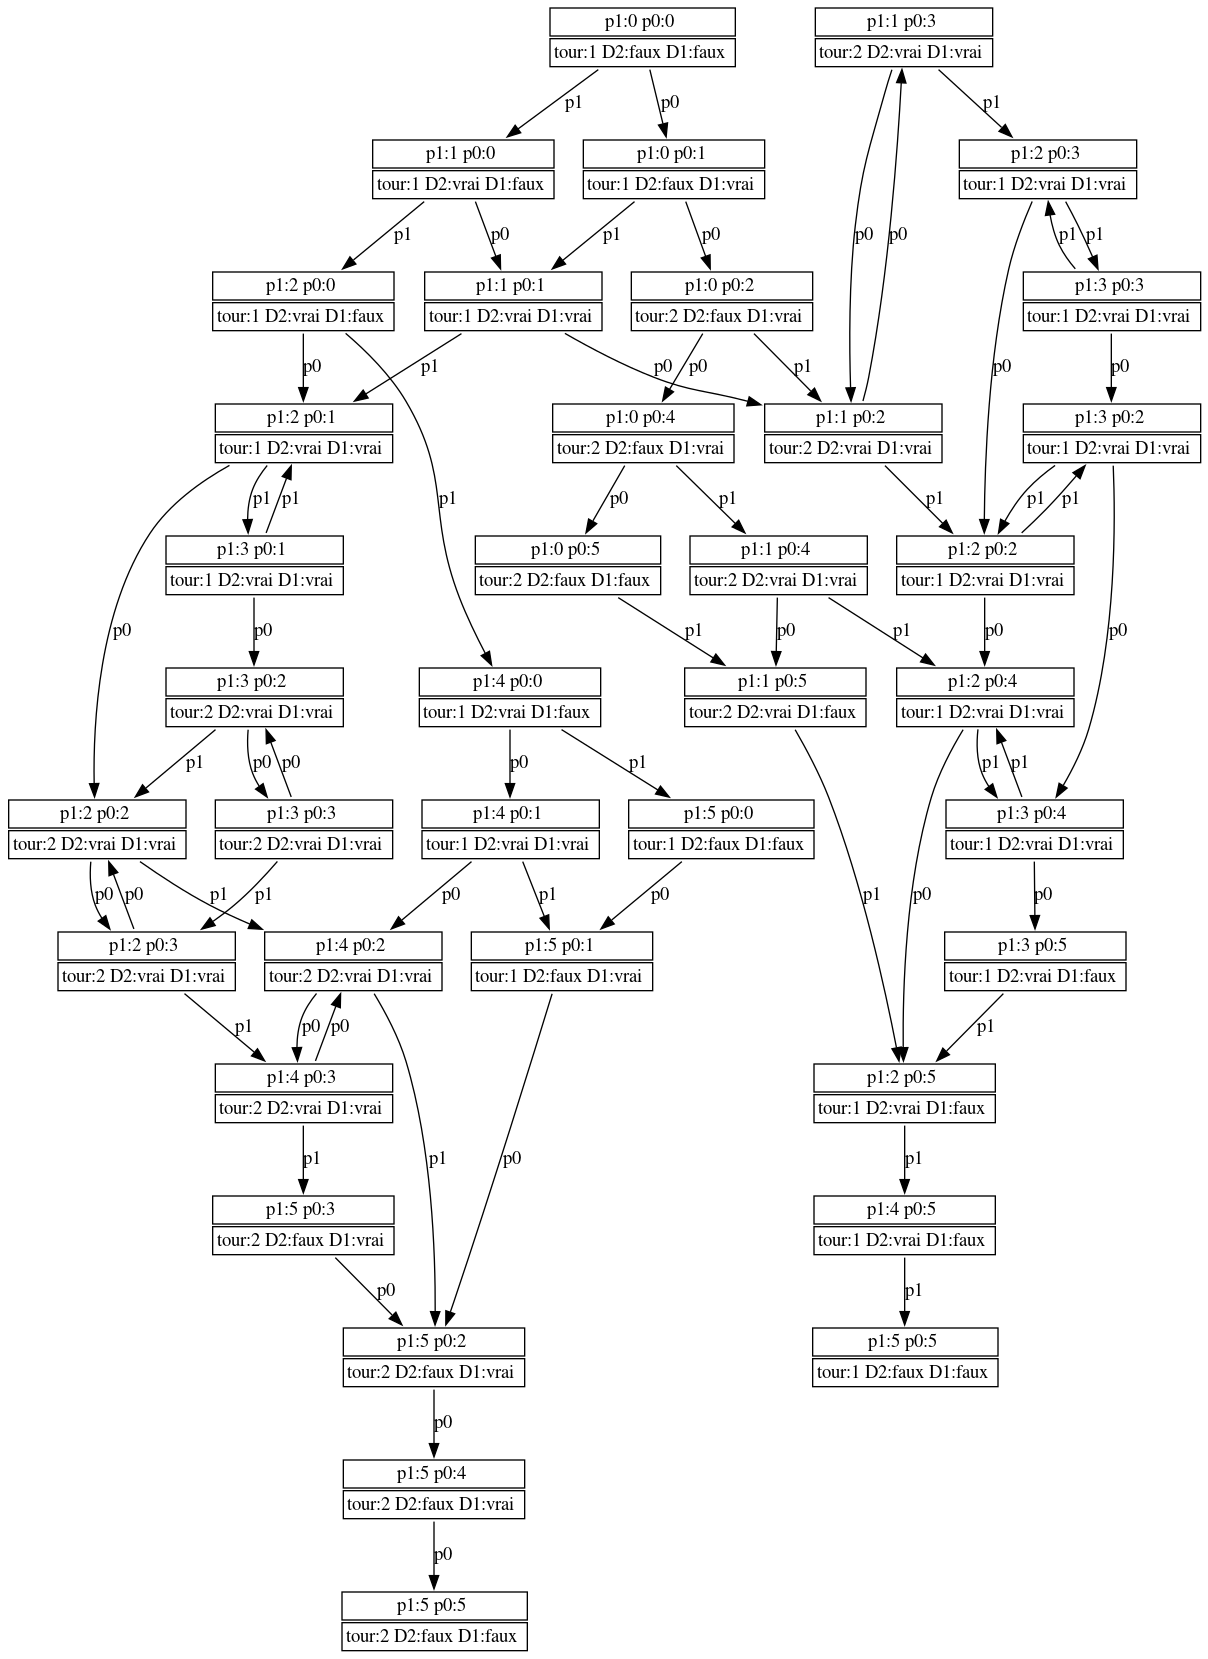
\includegraphics[width=\linewidth]{graphPeterson.png}
      \caption{Peterson graph}
      \label{fig:peterson}
  \end{figure}
\end{itemize}
\newpage


\subsubsection{Example 2}
We will use an algorithm with a decide to display how it works when one process has to decide a variable.
\begin{itemize}
  \item \textbf{CALODS:}
  \begin{lstlisting}
  type int = { 1, 2 }
  var int tmp = 1

  proc process_decide(){
   if (tmp == 1){
     decide 1
   } else {
     decide 2
   }
  }

  proc update_tmp() {
    tmp = 2
  }

  run process_decide() || update_tmp()
  \end{lstlisting}

  \item \textbf{ILODS:}
  \begin{lstlisting}
  type int = { 1, 2 }
  var tmp = 1

  = process_decide () =
  0: {jump if tmp == 1 to next, goto 3}
  1: {decide 1, finish}
  2: {move, goto 4}
  3: {decide 2, finish}
  4: {empty, eof}
 
  = update_tmp () =
  0: {tmp = 2, next}
  1: {empty, eof}
 
  parallel:
  call process_decide -> {}
  call update_tmp -> {}  
  \end{lstlisting}

  \item \textbf{Graph:} The graph is presented in figure 2.
  \begin{figure}
    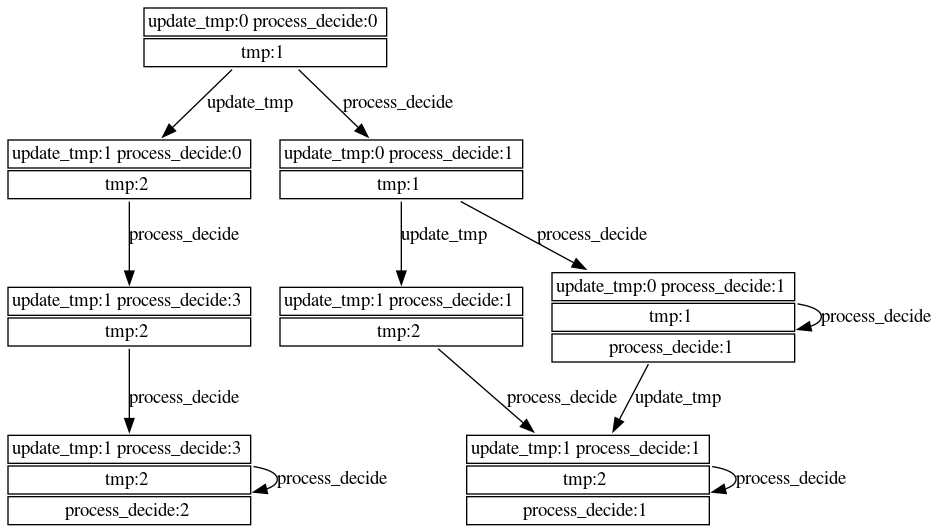
\includegraphics[width=\linewidth]{graphDecide.png}
      \caption{Decide graph}
      \label{fig:decide}
  \end{figure}
\end{itemize}

\newpage

\section{Conclusion}
We have learnt a lot of stuff through this project:
\begin{itemize}
  \item It helps us improve our understanding of distributed algorithms and the consensus problem.
  \item It allows us to write a kind of research paper about the work we have done.
  \item We confronted our understanding of the OCaml language with a real project.
  \item This project forced us to try to write a maintainable code other people will read.
\end{itemize}
Finally, we want to thank Mr. Sangnier and Mr Laroussinie for their help, their advises and the time they take for us.

\end{document}

